\documentclass{article}
\usepackage{graphicx}
\usepackage{hyperref}
\usepackage{caption}
\usepackage{subcaption}
\usepackage{mathtools}
\usepackage[dutch]{babel}

\begin{document}

\begin{center}
	\huge{Wiskunde in Kunst}\\
	\LARGE{Opdracht 9} \\
	
	\vspace{2cm}
	
	\Large{De Gulden snede}\\
	
	\vfill
	
	\begin{figure}[Hh]
		\centering
		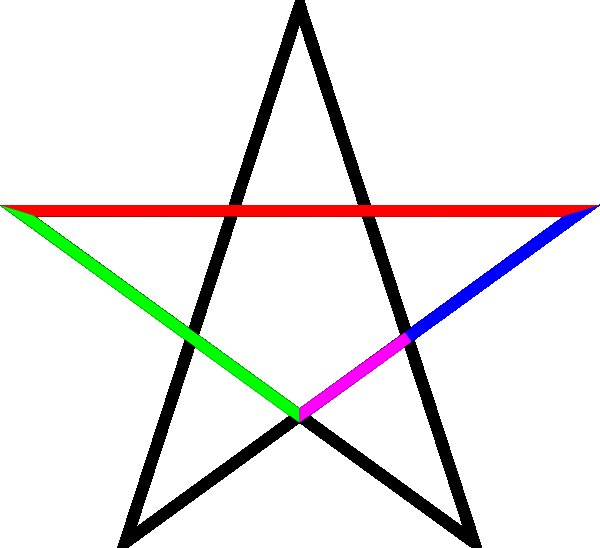
\includegraphics[width=\textwidth]{Pentagram-phi.jpg}
	\end{figure}
	
	\vfill
	\Large{Marcelo Dias Avelino} \hfill \large{0840416}
\end{center}

\thispagestyle{empty} % Remove page numbering

\pagebreak

\setcounter{page}{1} % Start counting pages here

\section{De gulden snede}

De gulden snede is een bekende verhouding in de wiskunde. Het houdt in dat bij twee lengtes, de verhouding tussen hun optelling en de grootste waarde gelijk is aan de verhouding tussen beide lijnen, zoals afgebeeld in Figuur \ref{fig:ratio-lines}. In dit geval is de verhouding tussen \( \frac{a+b}{a} \) gelijk aan \( \frac{a}{b} \). Dit verhouding wordt aangegeven met de griekse letter \(\varphi\) (phi) en staat gelijk aan \(\varphi = \frac{1+\sqrt{5}}{2} \approx 1.6180339887\). 

De wiskundige eigenschappen van dit getal worden als sinds de oudheid bestudeerd, maar het heeft de term \textit{gulden snede} pas in de 19e eeuw gekregen. Het vroegst bekende studie van dit getal stemt uit de tijd van Oude Griekland. De grieken waren begonnen met het bestuderen van de gulden snede vanwege zijn regelmatig verschijning in de geometrie en zijn een belangrijkheid om pentagrammen en pentagonnen te tekenen. De griekse wiskundig Euclides heeft in zijn meetkundig en rekenkundig verzamelwerk, de \textit{Elementen}, de eerste bekende definitie van wat nu bekend staat als de gulden sneden. Euclides beschreef het als ``Een rechte lijn is zogenaamd gesneden in de extreme en gemiddelde verhouding wanneer, zoals het gehele lijn staat voor de grootste segment, zo staat de grotere tot de kleinere.''. Door het gehele boek wordt de gulden snede gebruikt bij meerdere stellingen en hun bewijs. De verhouding was verder onderzocht in het boek \texit{De divina proportione} (De goddelijke properties) van de italianse wiskundig Fra Luca Bartolomeo de Pacioli, een mede-collaborateur van Leonardo da Vinci en een van de oorspronkelijk bijdragers aan het vakgebied van accountancy. Dit boek beschrijft de gulden snede vanuit een wiskundig inkijk hoek en bestudeert ook polygonen, een figuur in een plat vlak gevormd door rechte lijnen. Sinds de 20e eeuw is de gulden snede gepresenteerd door de letter \(\varphi\), genoemd naar de griekse beeldhouwer Phidias, die de gulden snede gebruikte in zijn kunst. Het wordt ook gepresenteerd door de letter \(\tau\) (tau), die `snijden' betekent.


\begin{figure}[Hh]
		\centering
		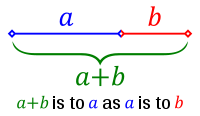
\includegraphics[width=0.35\textwidth]{golden-ratio-line.png}
		\caption{De verhouding tussen twee lengtes.}
		\label{fig:ratio-lines}
	\end{figure}

\end{document}
